\documentclass[10pt,a4paper]{article}
\usepackage[margin=13mm]{geometry}
\usepackage{tikz}
\setlength{\parindent}{0pt}
\begin{document}
{\Large\bfseries BFS and DFS: three worked examples}\par\smallskip
Start at $A$ and consider neighbors alphabetically. BFS marks on enqueue; DFS enters the first unvisited neighbor.\par\medskip
\textbf{1. Diamond and tail}\par\smallskip
\begin{minipage}[t]{0.31\textwidth}\textbf{Input graph}\par
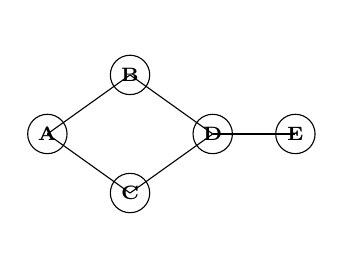
\begin{tikzpicture}[x=1cm,y=1cm]
  \path[use as bounding box] (-0.25,-1.35) rectangle (3.45,1.35);
  \tikzset{v/.style={circle,draw,minimum size=5mm,inner sep=0pt,font=\scriptsize\bfseries}}
  \draw (0.00,0.00)--(1.05,0.75);
  \draw (0.00,0.00)--(1.05,-0.75);
  \draw (1.05,0.75)--(2.10,0.00);
  \draw (1.05,-0.75)--(2.10,0.00);
  \draw (2.10,0.00)--(3.15,0.00);
  \node[v] at (0.00,0.00) {A};
  \node[v] at (1.05,0.75) {B};
  \node[v] at (1.05,-0.75) {C};
  \node[v] at (2.10,0.00) {D};
  \node[v] at (3.15,0.00) {E};
\end{tikzpicture}
\end{minipage}\hfill
\begin{minipage}[t]{0.31\textwidth}\textbf{BFS tree}\par
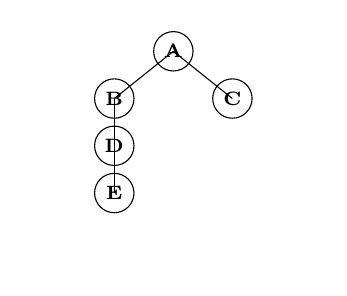
\begin{tikzpicture}[x=1cm,y=1cm]
  \path[use as bounding box] (-0.10,-2.75) rectangle (3.60,0.30);
  \tikzset{v/.style={circle,draw,minimum size=5mm,inner sep=0pt,font=\scriptsize\bfseries}}
  \draw (1.75,0.00)--(1.00,-0.60);
  \draw (1.75,0.00)--(2.50,-0.60);
  \draw (1.00,-0.60)--(1.00,-1.20);
  \draw (1.00,-1.20)--(1.00,-1.80);
  \node[v] at (1.00,-1.80) {E};
  \node[v] at (1.00,-1.20) {D};
  \node[v] at (1.00,-0.60) {B};
  \node[v] at (2.50,-0.60) {C};
  \node[v] at (1.75,0.00) {A};
\end{tikzpicture}
\par\scriptsize Frontier: \texttt{[A] [B,C] [D] [E] []}
\end{minipage}\hfill
\begin{minipage}[t]{0.31\textwidth}\textbf{DFS tree}\par
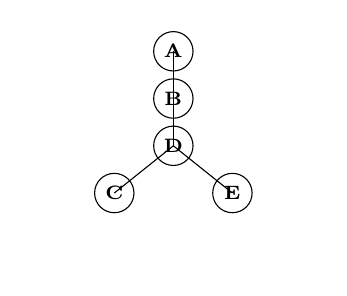
\begin{tikzpicture}[x=1cm,y=1cm]
  \path[use as bounding box] (-0.10,-2.75) rectangle (3.60,0.30);
  \tikzset{v/.style={circle,draw,minimum size=5mm,inner sep=0pt,font=\scriptsize\bfseries}}
  \draw (1.75,0.00)--(1.75,-0.60);
  \draw (1.75,-0.60)--(1.75,-1.20);
  \draw (1.75,-1.20)--(1.00,-1.80);
  \draw (1.75,-1.20)--(2.50,-1.80);
  \node[v] at (1.00,-1.80) {C};
  \node[v] at (2.50,-1.80) {E};
  \node[v] at (1.75,-1.20) {D};
  \node[v] at (1.75,-0.60) {B};
  \node[v] at (1.75,0.00) {A};
\end{tikzpicture}
\par\scriptsize Visit order: A, B, D, C, E
\end{minipage}\par
\vspace{5mm}\hrule\vspace{5mm}
\textbf{2. Shared neighbor}\par\smallskip
\begin{minipage}[t]{0.31\textwidth}\textbf{Input graph}\par
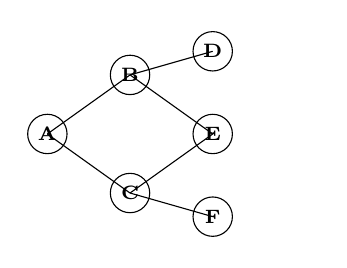
\begin{tikzpicture}[x=1cm,y=1cm]
  \path[use as bounding box] (-0.25,-1.35) rectangle (3.45,1.35);
  \tikzset{v/.style={circle,draw,minimum size=5mm,inner sep=0pt,font=\scriptsize\bfseries}}
  \draw (0.00,0.00)--(1.05,0.75);
  \draw (0.00,0.00)--(1.05,-0.75);
  \draw (1.05,0.75)--(2.10,1.05);
  \draw (1.05,0.75)--(2.10,0.00);
  \draw (1.05,-0.75)--(2.10,0.00);
  \draw (1.05,-0.75)--(2.10,-1.05);
  \node[v] at (0.00,0.00) {A};
  \node[v] at (1.05,0.75) {B};
  \node[v] at (1.05,-0.75) {C};
  \node[v] at (2.10,1.05) {D};
  \node[v] at (2.10,0.00) {E};
  \node[v] at (2.10,-1.05) {F};
\end{tikzpicture}
\end{minipage}\hfill
\begin{minipage}[t]{0.31\textwidth}\textbf{BFS tree}\par
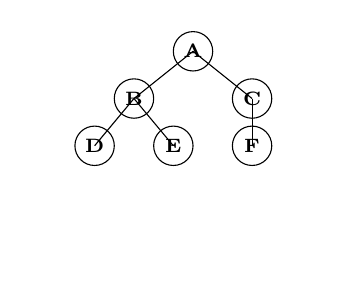
\begin{tikzpicture}[x=1cm,y=1cm]
  \path[use as bounding box] (-0.10,-2.75) rectangle (3.60,0.30);
  \tikzset{v/.style={circle,draw,minimum size=5mm,inner sep=0pt,font=\scriptsize\bfseries}}
  \draw (2.00,0.00)--(1.25,-0.60);
  \draw (2.00,0.00)--(2.75,-0.60);
  \draw (1.25,-0.60)--(0.75,-1.20);
  \draw (1.25,-0.60)--(1.75,-1.20);
  \draw (2.75,-0.60)--(2.75,-1.20);
  \node[v] at (0.75,-1.20) {D};
  \node[v] at (1.75,-1.20) {E};
  \node[v] at (1.25,-0.60) {B};
  \node[v] at (2.75,-1.20) {F};
  \node[v] at (2.75,-0.60) {C};
  \node[v] at (2.00,0.00) {A};
\end{tikzpicture}
\par\scriptsize Frontier: \texttt{[A] [B,C] [D,E,F] []}
\end{minipage}\hfill
\begin{minipage}[t]{0.31\textwidth}\textbf{DFS tree}\par
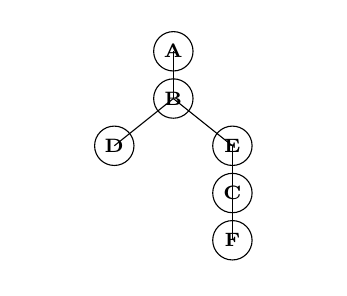
\begin{tikzpicture}[x=1cm,y=1cm]
  \path[use as bounding box] (-0.10,-2.75) rectangle (3.60,0.30);
  \tikzset{v/.style={circle,draw,minimum size=5mm,inner sep=0pt,font=\scriptsize\bfseries}}
  \draw (1.75,0.00)--(1.75,-0.60);
  \draw (1.75,-0.60)--(1.00,-1.20);
  \draw (1.75,-0.60)--(2.50,-1.20);
  \draw (2.50,-1.20)--(2.50,-1.80);
  \draw (2.50,-1.80)--(2.50,-2.40);
  \node[v] at (1.00,-1.20) {D};
  \node[v] at (2.50,-2.40) {F};
  \node[v] at (2.50,-1.80) {C};
  \node[v] at (2.50,-1.20) {E};
  \node[v] at (1.75,-0.60) {B};
  \node[v] at (1.75,0.00) {A};
\end{tikzpicture}
\par\scriptsize Visit order: A, B, D, E, C, F
\end{minipage}\par
\vspace{5mm}\hrule\vspace{5mm}
\textbf{3. Two routes}\par\smallskip
\begin{minipage}[t]{0.31\textwidth}\textbf{Input graph}\par
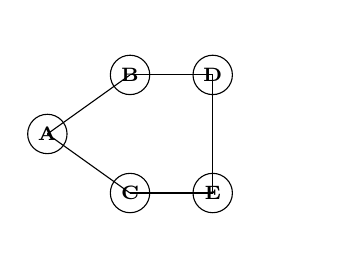
\begin{tikzpicture}[x=1cm,y=1cm]
  \path[use as bounding box] (-0.25,-1.35) rectangle (3.45,1.35);
  \tikzset{v/.style={circle,draw,minimum size=5mm,inner sep=0pt,font=\scriptsize\bfseries}}
  \draw (0.00,0.00)--(1.05,0.75);
  \draw (0.00,0.00)--(1.05,-0.75);
  \draw (1.05,0.75)--(2.10,0.75);
  \draw (1.05,-0.75)--(2.10,-0.75);
  \draw (2.10,0.75)--(2.10,-0.75);
  \node[v] at (0.00,0.00) {A};
  \node[v] at (1.05,0.75) {B};
  \node[v] at (1.05,-0.75) {C};
  \node[v] at (2.10,0.75) {D};
  \node[v] at (2.10,-0.75) {E};
\end{tikzpicture}
\end{minipage}\hfill
\begin{minipage}[t]{0.31\textwidth}\textbf{BFS tree}\par
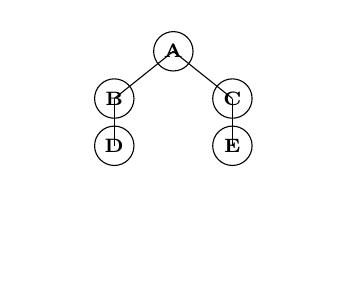
\begin{tikzpicture}[x=1cm,y=1cm]
  \path[use as bounding box] (-0.10,-2.75) rectangle (3.60,0.30);
  \tikzset{v/.style={circle,draw,minimum size=5mm,inner sep=0pt,font=\scriptsize\bfseries}}
  \draw (1.75,0.00)--(1.00,-0.60);
  \draw (1.75,0.00)--(2.50,-0.60);
  \draw (1.00,-0.60)--(1.00,-1.20);
  \draw (2.50,-0.60)--(2.50,-1.20);
  \node[v] at (1.00,-1.20) {D};
  \node[v] at (1.00,-0.60) {B};
  \node[v] at (2.50,-1.20) {E};
  \node[v] at (2.50,-0.60) {C};
  \node[v] at (1.75,0.00) {A};
\end{tikzpicture}
\par\scriptsize Frontier: \texttt{[A] [B,C] [D,E] []}
\end{minipage}\hfill
\begin{minipage}[t]{0.31\textwidth}\textbf{DFS tree}\par
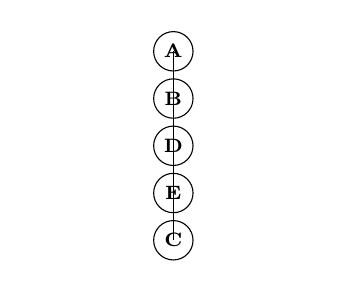
\begin{tikzpicture}[x=1cm,y=1cm]
  \path[use as bounding box] (-0.10,-2.75) rectangle (3.60,0.30);
  \tikzset{v/.style={circle,draw,minimum size=5mm,inner sep=0pt,font=\scriptsize\bfseries}}
  \draw (1.75,0.00)--(1.75,-0.60);
  \draw (1.75,-0.60)--(1.75,-1.20);
  \draw (1.75,-1.20)--(1.75,-1.80);
  \draw (1.75,-1.80)--(1.75,-2.40);
  \node[v] at (1.75,-2.40) {C};
  \node[v] at (1.75,-1.80) {E};
  \node[v] at (1.75,-1.20) {D};
  \node[v] at (1.75,-0.60) {B};
  \node[v] at (1.75,0.00) {A};
\end{tikzpicture}
\par\scriptsize Visit order: A, B, D, E, C
\end{minipage}\par
\end{document}
